The final product will allow the user to generate multiple types of landscapes by adjusting generation settings. And consecutively navigate through a rendering of the generated world. 

\subsection{Generation}

\subsubsection{Existing algorithm}

\begin{figure}[H]
	\centering
	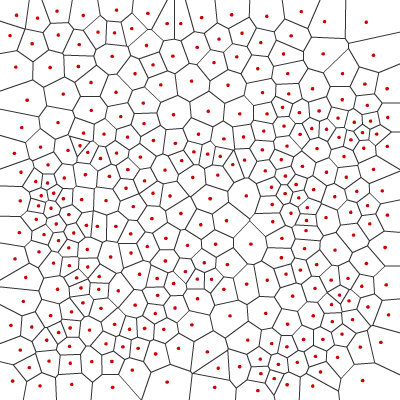
\includegraphics[width=\linewidth]{voronoi}
	\caption{Voronoi diagram}
	\label{fig:voronoi}
\end{figure}

The existing algorithm presented by Patel\cite{redblob} generates landscapes or maps more closely related to what is represented, as opposed to some mathmatical function leading to a randomized height map. All generated maps are islands and are generated by modifying a partitioning of the map in polygons. This partitioning is a Voronoi diagram ~\ref{fig:voronoi}. It is acquired by first generating points, the distance from anywhere within the resulting polygons to the associated point will allways be smaller than the distance to any other point.

We can imagine two graphs being used, one which shows adjacency relations between polygons and one which contains the actual edges of the resulting map. But because of the one-to-one relationship between edges in both these graphs Patel\cite{redblob} stored the edges of the map only once and simply added attributes for which polygons they bordered.

The next step is to divide the map in land and water. Water on the edges of the map will be regarded as sea. This affects the elevation as it is directly dependant on the distance from the coast. If water was generated inland these polygons can be regarded as lakes and are higher than the sea due to the fact that elevation is dependant on the distance to the sea, this allows easy generation of rivers downhill which will allways end up in another body of water. Additionally, moisture at a certain point in the map can be determined by distance to water and combined with elevation to allow for a relatively easy assignment of biomes.

Lastly some sort of noise can be used to litterally blur the lines of the underlying structure while still maintaining the useful properties of this method of generation for pathfinding and other game related mechanics. Figure~\ref{fig:biomes} shows an example of what this type of noise can accomplish.

\newlength{\imagewidth}
\settowidth{\imagewidth}{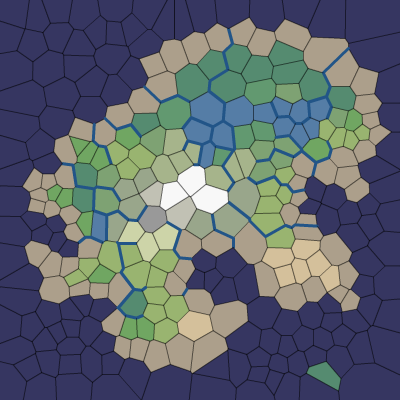
\includegraphics{biomes}}

\begin{figure}[H]
	\centering
	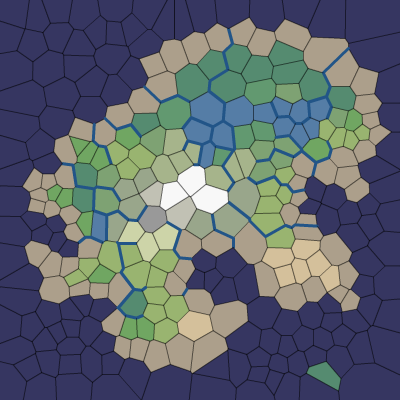
\includegraphics[trim=0 0 0.5\imagewidth{} 0, clip,width=0.45\linewidth]{biomes}
	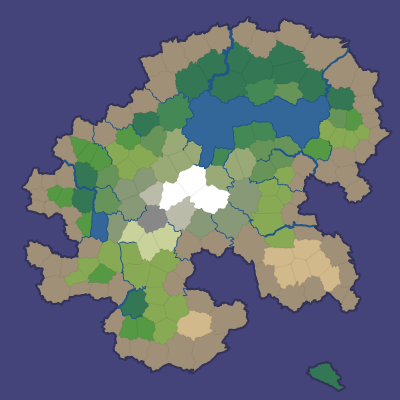
\includegraphics[trim=0.5\imagewidth{} 0 0 0, clip,width=0.45\linewidth]{biomes-noisy}
	\caption{Edge noise}
	\label{fig:biomes}
\end{figure}

\subsubsection{Generation extention}

In addition to the existing algorithm we would like to modify it such that multiple peaks can be generated. We would allow elevation to vary instead of being solely dependant on distance to water. We do however want to maintain the useful properties this presented with respect to rivers and such. A way to do this for rivers specifically is to maintain bodies of water wherever the elevation is less than expected based on distance to the shore. It does not seem unreasonable to expect water to accumulate in such a place. 

In fact the existing algorithm only allows for multiple high points to occur due to water placement. Figure~\ref{fig:map-3d} shows that two seperate ridges formed on either side of the lake. Another option would be to apply post-processing to adjust heights that do not affect placement of rivers and such before assigning biomes.

\subsection{Visualisation}

\subsubsection{Land}

When rendering the landscapes we will want to obviously texture land in accordance with the biomes. To add some diversity we would like to add some grass or other simple vegetation.

\subsubsection{Water}

Bodies of water will be modelled as animated (preferably reflective) surfaces. Rivers will be given the same representation and be positioned slightly lower but follow the general shape of the associated edge.

\subsubsection{NPC's}

To illustrate the usefulness of the generation method we would introduce some non-player characters to move through the generated world, similarly to Braitenberg vehicles. Their path will be influenced by biomes or affected by obstructions such as rivers and mountains.